\section{Results II: Adversarial Red-Team, Off-Body Coupling, and the Supervised Baseline}
\label{sec:results_redteam}

The within-session and same-rig cross-session results of \Cref{sec:results_main} establish that the trained Phase~G verifier separates genuine chain-coupled captures from temporally mispaired or shuffled emissions essentially without error. Those results, however, are constructed entirely from \emph{real} captures: the ``wrong-$E$'' negatives are real frames paired with the wrong emission. A verifier that only rejects mispaired-but-real captures says nothing about an adversary who synthesizes a forged capture $C_{\mathrm{fake}}$ explicitly conditioned on the real target emission $E_{\mathrm{target}}$. This section reports the system's behaviour against such a learned attacker, dissects \emph{where} in the image the discriminative signal lives, and characterizes a separately trained supervised baseline together with a fine-grained perturbation-sensitivity sweep. Throughout, two scope guards apply and are stated wherever a number is quoted: all evaluations are \emph{same-rig} (the single D2/V10 rig, one performer, two sessions) --- they do \emph{not} establish cross-rig, cross-camera, cross-projector, or cross-subject behaviour --- and the only \emph{trained} attacker is F-A~v1. The stronger F-A~v2 attacker is a design specification only; it is not trained, its trainer code does not exist, and nothing here should be read as a robustness claim against a strong or adaptive forger.

\subsection{Stage 0: a learned forger (F-A v1) is caught at every checkpoint}
\label{sec:redteam_stage0}

The red-team attacker, designated F-A~v1, is a learned editor that produces fake captures conditioned on a target emission. It is a 42.3M-parameter ControlNet-style \texttt{EditorControlNet}~\cite{zhang2023controlnet} built over a ConvNeXt-Tiny source encoder~\cite{liu2022convnext}: a $9$-channel spatial hint ($E_{\mathrm{target}}\,\|\,E_{\mathrm{source}}\,\|\,\Delta$) plus a $2$-channel coordinate grid is injected via zero-convolution adapters at four ConvNeXt scales. It was trained for \num{100000} steps ($\approx$\,\SI{28}{\hour}\,\SI{18}{\minute}; effective batch size $16$ on $8\times$ A100) against a pool of \emph{surrogate} binders (exp001c and e1-bf16 as training surrogates, with e2, e3r and an ablation family held out), so that it never received gradients from the Phase~G verifier itself. This separation is enforced as policy: Phase~G is reserved for final evaluation and is never used for attacker training, validation, checkpoint selection, or curriculum.

The headline Stage~0 result is that the Phase~G verifier rejects F-A~v1 forgeries at frame-level AUROC $=1.000$ for the real-correct vs.\ fake-correct contrast (genuine capture vs.\ forged capture, both paired with the correct $E_{\mathrm{target}}$), in \emph{both} sessions and at \emph{every} evaluated checkpoint --- steps 5k, 25k, 70k, and 100k --- on the standard held-out blocks (D2 $n=198$, V10 $n=200$). The attacker does not escape the verifier as it matures; its capacity to reproduce raw-capture realism plateaus while the verifier's separation remains saturated. We stress that this is a result about F-A~v1 specifically and is same-rig only.

A crucial nuance prevents a trivial reading of this result. One might suspect F-A~v1 is caught merely because it ignores the conditioning emission --- i.e.\ that it never learned to couple its output to $E_{\mathrm{target}}$ at all, so the verifier is simply detecting an absent hint. This is \emph{not} the case. By step 100k, F-A~v1 has demonstrably learned partial target-$E$ coupling: a forgery paired with its true $E_{\mathrm{target}}$ scores measurably better than the same forgery paired with a shuffled emission, with the fake-correct vs.\ fake-shuffled AUROC reaching $0.9927$ on D2 and $0.9295$ on V10. This coupling strengthens monotonically over training (D2: $0.609\!\to\!0.818\!\to\!0.967\!\to\!0.993$ across 5k/25k/70k/100k; V10: $0.585\!\to\!0.748\!\to\!0.870\!\to\!0.930$), confirming the editor is genuinely conditioning on $E$. F-A~v1 is therefore caught not for lacking emission structure, but for failing the \emph{real-capture conditional distribution}: its outputs do not reproduce the raw-capture realism, the fine chain-coupled statistics, and the source-leakage-free structure of genuine BayerRG8 frames. The held-out binder evaluation corroborates a \emph{soft} white-box specialization rather than catastrophic overfitting: the training-family binders score F-A~v1 output roughly \SI{3}{\decibel} better than held-out binders ($\approx$\,\SI{5}{\decibel} training target-gap vs.\ $\approx$\,\SI{1.7}{\decibel} held-out), yet the held-out family still ranks the true target first in $100\%$ of cases.

\paragraph{Probe saturation and decomposition deferral.}
We attempted to decompose \emph{why} the verifier separates F-A~v1 so cleanly by fitting logistic probes on Stage~0 diffusion features. Three feature families --- a Raw set (4 conditional MSEs), a Coupling set (3 contrasts), and their union (7 features) --- all saturate at AUROC $=1.000$ on the headline split (train on fakes at 5k/25k/70k, test on fakes at 100k; $n_{\mathrm{train}}=1272$, $n_{\mathrm{test}}=160$), and the saturation persists under leave-one-checkpoint-out cross-validation across all four checkpoints. Because every probe is perfect, F-A~v1 is simply too easy a target to support a meaningful feature-level decomposition; the deeper decomposition modes are deferred until a harder target (a trained F-A~v2) exists. We flag this as a deferral, not a completed analysis.

\paragraph{Cross-verifier robustness.}
A leave-one-session-out cross-verifier check confirms the forgeries remain detectable when scored by a verifier trained on only one session. The harder within-fake discrimination (fake-correct vs.\ fake-shuffled) degrades modestly out-of-distribution --- a D2-only verifier scores held-out V10 fakes at $0.8588$ (vs.\ $0.9295$ for the combined verifier), while a V10-only verifier holds D2 at $0.9927$ --- indicating that part of the verifier's coupling signal is session-specific and that F-A~v1 exploits that session-specific weakness. The real-pair coupling contrasts (real-correct vs.\ shuffled, real-correct vs.\ source) remain at AUROC $=1.000$ in all six (session $\times$ verifier) cells, so the core verification signal on genuine captures is intact across the ablation.

\subsection{Attacker non-convergence under continued training}
\label{sec:redteam_progression}

The visualization corpus (\num{9735} frames across D2 and V10) makes the non-convergence behaviour directly legible. Scoring a fixed captured frame against synthetic emissions drawn from successive attacker training steps, the substrate-verification \emph{excess} panel --- the per-pixel residual above the full-corpus p99.9 floor --- stays strongly red at every maturity. The mean synthetic excess-red area declines only modestly across training ($67.4\% \to 59.2\% \to 55.1\% \to 52.4\%$ at steps 5k/25k/70k/100k), while the genuine condition holds at a mean real-correct red area of $0.018\%$. \Cref{fig:attacker_progression} shows this progression for a single frame and reference: as the attacker matures its forgeries become marginally less anomalous, but the chain-coupled signature does not vanish. We emphasize that this is the F-A~v1 attacker; the result demonstrates that \emph{this} attacker does not converge to escape under continued training, not that no attacker could.

\begin{figure}[t]
\centering
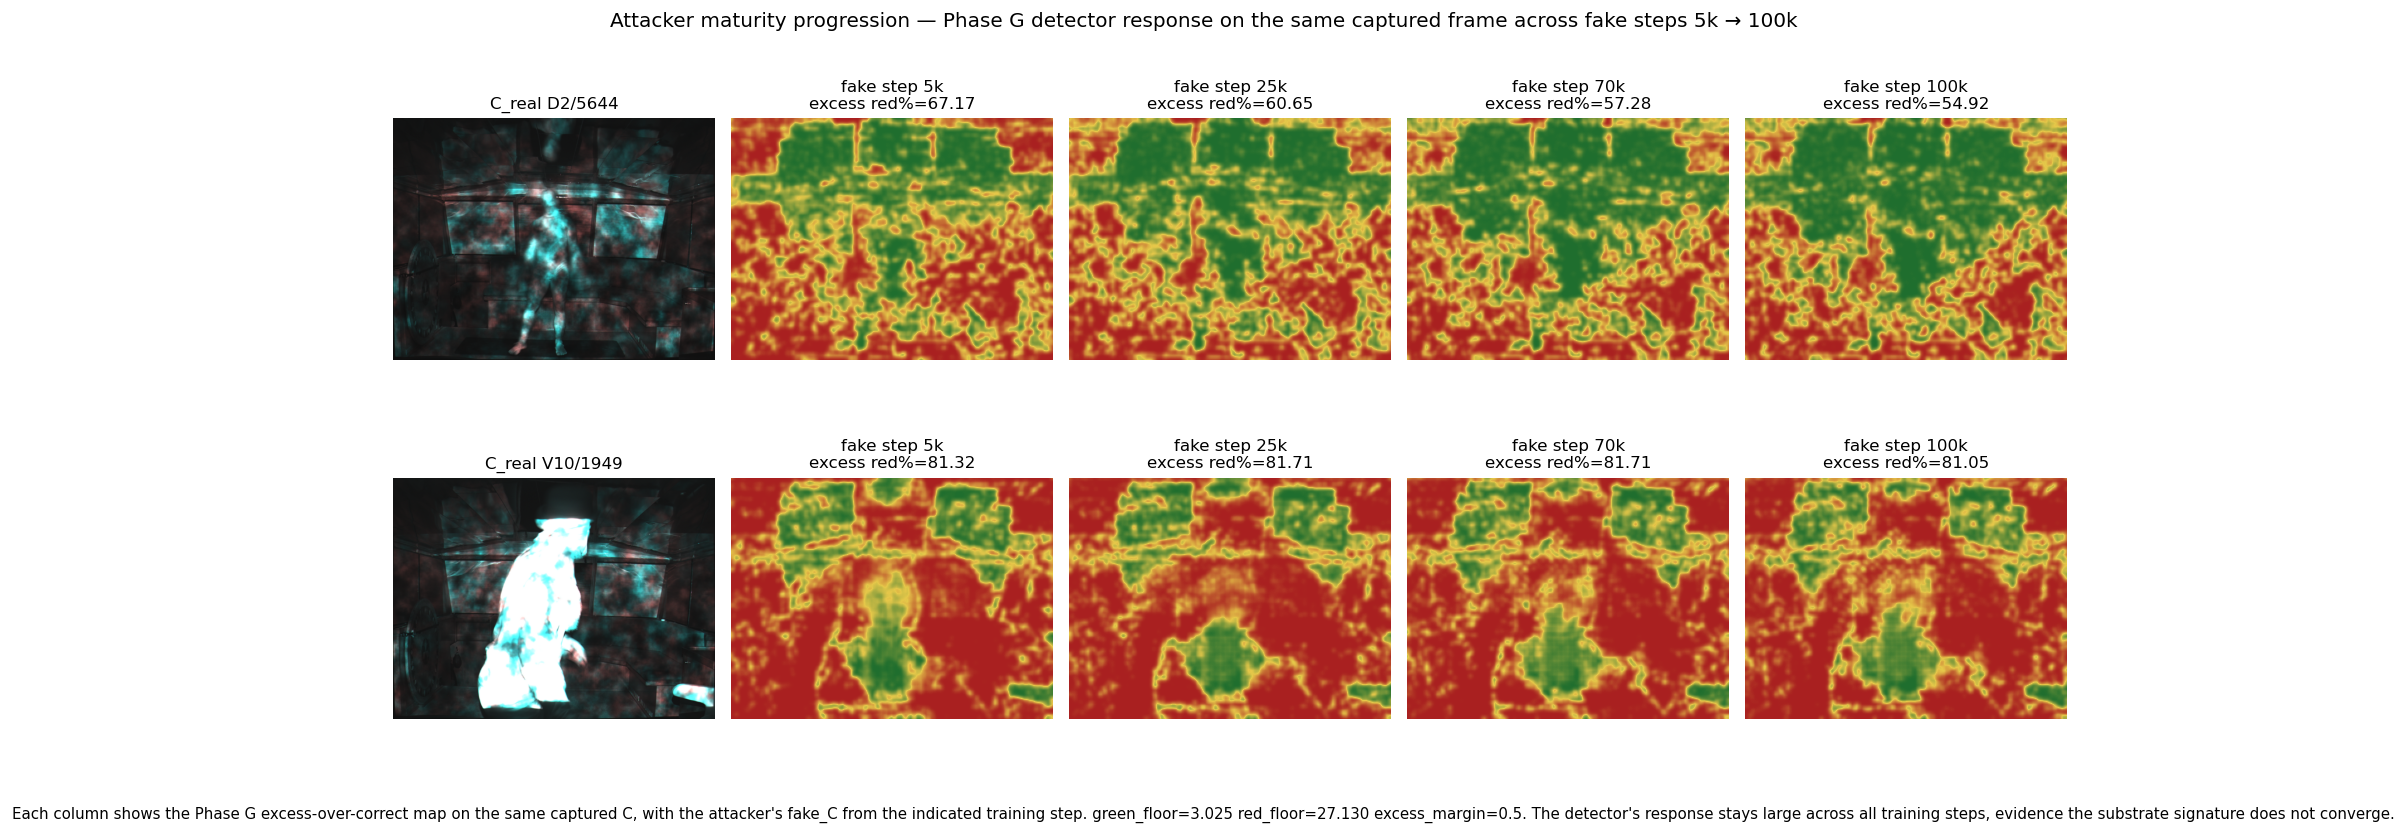
\includegraphics[width=\linewidth]{figures/fig_attacker_progression.png}
\caption{Attacker non-convergence (red-team). For a single captured frame $C$ and a single per-session reference, the synthetic emission is taken from F-A~v1 training steps 5k, 25k, 70k, and 100k. The substrate-verification excess panel remains strongly red at every step (mean excess red area $67.4 \to 59.2 \to 55.1 \to 52.4\%$), while the genuine condition holds at mean real-correct red area $0.018\%$. Residual coverage decreases only modestly as the attacker matures, indicating the chain-coupled signature does not converge under continued training of this attacker (F-A~v1). Green floor $=$ full-\num{9735} p95, red floor $=$ p99.9, excess margin $0.5$, common thresholds across all steps; no per-frame normalization.}
\label{fig:attacker_progression}
\end{figure}

\subsection{Where the discriminative signal lives: off-body, not on-body}
\label{sec:redteam_offbody}

A causal-ablation study asks which spatial region of the capture carries the signal the verifier uses to reject F-A~v1. The answer required correcting an early methodological error, and the correction inverted the conclusion; we report both readings because the inversion is itself instructive.

\paragraph{The variance-box reading and its failure.}
The first ablation masked the image into a ``body'' region and an ``off-body'' region using a variance-box heuristic (a $32\times32$ sliding-window variance with a p75 threshold, taking the largest vertically-extended connected component with a $10\%$ bounding-box expansion). Replacing the off-body region (condition E2, ``body only'') retained AUROC in the range $0.973$--$0.997$ on D2 and $0.983$--$0.995$ on V10, while replacing the body (condition E3, ``off-body only'') gave a lower $0.789$--$0.896$ (D2) / $0.926$--$0.977$ (V10). Read naively, this suggested ``body-region primacy.'' Visual inspection of the variance-box masks revealed the flaw: the heuristic ``body'' mask captured the body \emph{plus} adjacent high-variance non-body content --- projector patterns cast on the background, scene structure, and sensor frame edges. The variance box is a poor proxy for the subject silhouette precisely because the projected chain-coupled illumination makes static background regions high-variance.

\paragraph{The proper-segmentation reading inverts the conclusion.}
Re-running the identical ablation with true person silhouettes from a Mask R-CNN ResNet50-FPN segmenter \cite{he2017maskrcnn} (COCO weights; largest connected component with morphological close/open; \num{106} of \num{120} frames usable after dropping 14 pathological frames, an $11.7\%$ combined rate; per-session minimum 50/56) \emph{inverts} the finding. With proper segmentation, the body-only condition E2$_{\mathrm{seg}}$ collapses to AUROC $0.009$--$0.538$, while the off-body-only condition E3$_{\mathrm{seg}}$ reaches AUROC $=1.000$ across all twelve (session $\times$ condition) cells (the conditions being fake at 5k/25k/70k/100k, shuffled-$E$, and cross-session-$E$, for each of D2 and V10). All twelve cells classify as ``body alone insufficient'' under a decision tree frozen before the analysis. The paired hierarchical-bootstrap $\Delta$AUROC (E2$_{\mathrm{seg}}$ minus the variance-box E2) is large and its $95\%$ CI excludes zero in every cell --- e.g.\ D2 fake-5k $\Delta = -0.984$ $[-0.998, -0.964]$. An independent audit recomputed representative cells exactly (e.g.\ D2 fake-5k E2$\to$E2$_{\mathrm{seg}}$: $0.9924 \to 0.0088$) and returned a PASS verdict. \Cref{fig:segmentation} illustrates the ablation on a single frame.

\begin{figure}[t]
\centering
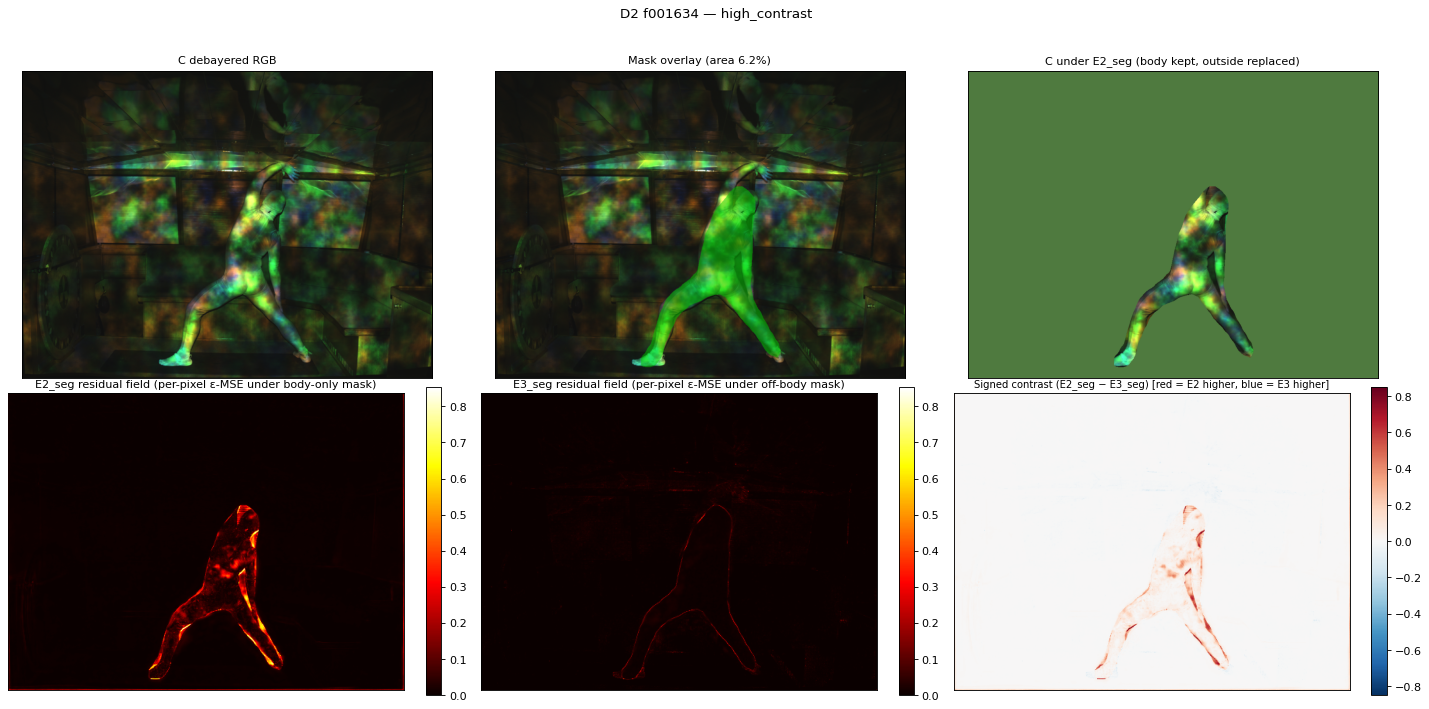
\includegraphics[width=\linewidth]{figures/fig_segmentation.png}
\caption{Where the discriminative signal lives: off-body, not on-body (segmentation ablation, frame D2 row 1634). Top row: debayered capture $C$, Mask R-CNN person mask (green overlay), and $C$ under the body-only ablation E2$_{\mathrm{seg}}$ (body kept, off-body replaced with per-channel inside-mask mean). Bottom row: E2$_{\mathrm{seg}}$ per-pixel residual field, E3$_{\mathrm{seg}}$ (off-body-only) residual field, and their signed contrast. Under proper Mask R-CNN segmentation, preserving only off-body content (E3$_{\mathrm{seg}}$) yields AUROC $=1.000$ across all conditions, while preserving only the body (E2$_{\mathrm{seg}}$) drops to chance or below (D2 fake AUROC $0.009$--$0.024$; $E$-perturbation $\approx 0.54$). This overturns an earlier variance-box reading and shows Phase~G's discrimination on F-A~v1 fakes resides in the off-body region. Scope caveat: analysis is over \num{106} usable frames and excludes the D2 block-2 supine-pose subset that Mask R-CNN segments unreliably ($11.7\%$ combined pathological rate; per-session minimum 50/56 usable).}
\label{fig:segmentation}
\end{figure}

\paragraph{Interpretation: likelihood overspread, not ``fakes look more real.''}
A striking feature of the inverted result is that the body-only AUROC falls \emph{below} chance on F-A~v1 fakes (D2 fakes $0.009$--$0.024$; V10 fakes $0.148$--$0.261$), meaning that under body-only masking, fake frames receive \emph{lower} anomaly scores than genuine frames. The correct framing is distribution-distance, not realism: F-A~v1 smooths body content, and its fake body region therefore lies in a region of Phase~G's conditional-likelihood landscape \emph{closer to the mode} than typical training-distribution real samples. This matches the overspread failure mode of likelihood-based out-of-distribution detection identified by Nalisnick et al.\ \cite{nalisnick2019} --- the reading most consistent with our measurements --- and we state it in those terms rather than as a claim that ``fakes look more real than real.'' The off-body reasoning is complementary: F-A~v1 does not perturb off-body content in a chain-coupled way, so the off-body region --- background scene, projection on static surfaces, and sensor frame edges --- retains the full discriminative chain-coupled signal and yields E3$_{\mathrm{seg}}$ AUROC $=1.000$.

\paragraph{The body signal is not absent --- it is at low spatial frequency.}
The ``body alone insufficient'' conclusion is specific to the $\lVert \hat{\epsilon}-\epsilon\rVert^2$ scoring function used by the verifier. The body region does carry a discriminative signal; it lives at low spatial frequencies that the residual-MSE score washes out under high-frequency dominance. Substituting a low-frequency scoring function (a Gaussian-blurred residual MSE, $\sigma = 4$) recovers body-only E2$_{\mathrm{seg}}$ AUROC $\approx 0.998$ (D2 $0.997$, V10 $0.998$), whereas $\lVert \hat{\epsilon}-\epsilon\rVert^2$ on the same masked region gives $\approx 0.30$--$0.41$ and a high-frequency residual is worse still ($\approx 0.21$--$0.32$). The correct claim is therefore narrow: residual-MSE body-only discrimination fails via OOD overspread, while a low-frequency body signal survives. We do not claim the body region is uninformative.

\paragraph{The relative-comparison test is unaffected and remains load-bearing.}
The absolute-MSE / OOD-overspread phenomenon above is orthogonal to a per-frame \emph{relative} chain-coupling test (EXP~6). In that test, each frame's correct emission is ranked against 50 random wrong emissions from the same session (with a $\pm 10$-frame temporal exclusion), giving 51 candidates per frame. The verifier ranks the correct $E$ first in $100\%$ of frames (top-1 $=1.000$, top-5 $=1.000$, mean rank $1.00$; $n=120$, D2$=60$ / V10$=60$). Because this test compares candidate emissions for a fixed capture rather than comparing absolute residual magnitudes across frames, it is immune to the overspread artifact and remains the load-bearing demonstration that Phase~G's signal is genuine chain-coupling.

\paragraph{Multi-method agreement on genuine captures.}
As a cross-check, the verifier-tier residuals can be compared against diagnostic representations on genuine frames (\Cref{fig:multimethod}). Two verifier-tier methods (Phase~G K2 and a binder residual) and two autoencoder-based diagnostic taps (AE-64f and AE-DGW) all report typical (green) residual on real-correct frames. The autoencoder methods are reported for cross-checking only and are explicitly labeled \textsc{Diagnostic}, not verifier-tier, because they exhibit weak coupling-specificity; quantitative claims rest on the per-method AUROC tables, not on the clipped display.

\subsection{A supervised baseline (Phase H): coarse-aware, fine-blind}
\label{sec:redteam_phaseh}

To contextualize the diffusion verifier against a conventional discriminative approach, we trained a small supervised CNN classifier (Phase~H) on $(C,E)$ input with real captures as positives and shuffled / perturbed-XOF captures as negatives. Phase~H is a coarse baseline with a known data-augmentation limitation, not a production verifier, and we report it as such.

\paragraph{It is emission-aware for coarse contrasts.}
An $E$-usage ablation on the converged checkpoint confirms Phase~H genuinely uses the emission for coarse discrimination: AUROC(target vs.\ shuffled) $=1.0000$ and AUROC(target vs.\ source) $=1.0000$ in both sessions (mean per-frame logits, D2: target $+4.897$, shuffled $-13.674$, source $-13.675$). The classifier cleanly separates the target emission from substantially different emissions. We note that AUROC(target vs.\ zero-$E$) reads $0.0$, but this is an out-of-distribution artifact --- zero-$E$ was never observed in training, and its mean logit ($+35.6$) sits far outside the in-distribution range --- so we do not cite it as a failure; the conclusions rest on the in-distribution target-vs-shuffled and target-vs-source contrasts.

\paragraph{It is blind to fine XOF perturbations.}
The same classifier does not resolve fine emission perturbations: Type~1 global BLAKE3-XOF bit-flips and Type~3 spatially-localized bit-flips score approximately at chance, while a Type~6 full-emission replacement is separated perfectly (AUROC $=1.0$). The canonical framing, which we adopt verbatim, is that ``the supervised CNN baseline is $E$-aware, but its learned evidence is coarse. It separates target emissions from substantially different emissions, but does not resolve fine XOF-level perturbations in this training regime.'' The distinction is one of contrast scale and perturbation family, not of abstract granularity.

\paragraph{The blindness is partly a label-locking artifact.}
A sampling audit identifies the proximate cause as per-frame label-locking: the epoch seed is fixed once at dataset construction and never refreshed, so each (session, row, index) tuple is permanently locked to a single role (positive, shuffled, or perturbed-with-a-specific-label). With 28 train-pool perturbation labels and a dataset of \num{2679} samples per epoch (positive $49.6\%$, shuffled $25.4\%$, perturbed $25.0\%$), only $\approx$\,17--33 unique frames back each perturbation label. Roughly half of all frames are never shown as a negative, and the model learns a per-frame label rather than per-condition discrimination. The recommended fix is to re-derive the epoch seed per epoch so frames rotate through all roles. We therefore attribute Phase~H's fine-blindness to the perturbation family combined with this augmentation deficiency, not to an intrinsic granularity ceiling.

\subsection{Item 1: fine-grained perturbation sensitivity of the diffusion verifier}
\label{sec:redteam_item1}

Finally, we probed whether the trained Phase~G diffusion verifier itself --- the load-bearing method --- exhibits the same coarse/fine structure. The Item~1 sweep ran 53 conditions $\times$ 2 sessions (D2 $n=198$, V10 $n=200$) against the main checkpoint at the five fixed eval timesteps with $K=4$ noise samples, augmenting the baseline conditions with 35 extended XOF perturbations. Per-condition AUROCs for the extended families are computed directly from the raw evaluation arrays; the shipped summary file covers only the baseline conditions.

The sweep is exploratory: per-condition AUROCs are reported descriptively, without multiple-comparisons correction across the 53 conditions; saturated separations (AUROC $=1.000$) lie far beyond any plausible multiplicity artifact, while near-chance values are read only as ``not detected,'' never as evidence of absence. The verifier confirms the same fine/coarse divide observed in Phase~H, now with a graded, frequency-dependent structure:
\begin{itemize}
  \item \textbf{Fine perturbations are near-chance.} Type~1 global bit-flips rise only at very large flip counts (D2: $k{=}1$ AUROC $0.503 \to k{=}4096$ AUROC $0.599$; V10: $0.503 \to 0.583$). Type~3 localized $8\times8$-region bit-flips in octave 2 stay near chance even at $k{=}256$ (D2 $0.506$, V10 $0.505$). We explicitly do \emph{not} claim Phase~G detects small-$k$ Type~1 or fine Type~3 flips.
  \item \textbf{Sensitivity is octave/persistence-dependent.} Low-frequency octave-0 perturbations are detectable while high-frequency octave-3 perturbations remain near chance: Type~2 oct-0 $k{=}64$ reaches $\approx 0.57$--$0.59$ vs.\ $\approx 0.503$ for oct-3; a Type~4 octave swap is perfect for oct-0 ($1.000$) but only $\approx 0.57$ for oct-3.
  \item \textbf{Gross perturbations are perfectly separable.} Full-emission replacement (Type~6), the wrong-$E$ offset, the octave-0 swap (Type~4), and the R-channel swap (Type~5) all reach AUROC $=1.000$ in both sessions; a B-channel swap is high but imperfect ($0.987$ D2 / $0.970$ V10) and is reported distinctly.
\end{itemize}
A renderer-calibration check passes (the Type~6 calibration condition matches the existing wrong-$E$ condition to $\approx 5\times 10^{-6}$ per-frame MSE), confirming the XOF$\to$render pipeline is deterministic and reproduces the baseline wrong-$E$ renderer. These sensitivities should be interpreted against the rendered-emission difference $\Delta E$: a very small XOF bit-flip may fall below the optical-relevance threshold, so its near-chance AUROC likely reflects an emission that is barely changed at the projector rather than a verifier deficiency. The graded result is consistent with the optical low-pass characterization of the substrate: the chain-coupled signal that survives projection and capture is the emission's low-frequency structure, and that is exactly where verifier sensitivity is highest.
